\graphicspath{{anexos/AnexoB-Diagrama-Clases-Completo/recursos/}}

\section{Diagrama de clases completo} \label{Anexo:diagrama-clases}

En este anexo incluimos el diagrama de clases completo, que se encuentra explicado detalladamente en la \autoref{sec:4:diseño} relativa al diseño del software del presente proyecto.

Este esquema puede ser visto en 4 partes: azul, amarillo/naranja, verde y rosa/magenta. Todas ellas emplean el principio de diseño software SOLID de segregación de la interfaz, que favorece el desacoplamiento del sistema; y el patrón de diseño \textit{Template Method}, que permite reutilizar código común reescribiendo únicamente aquellas partes diferenciadores de cada elemento concreto.

Por ejemplo, en la parte verde, relativa al paquete que representa el proceso de búsqueda VNS, se emplea el método \texttt{startExecution} como plantilla que emplea los demás métodos. En especial tenemos el método abstracto \texttt{vnsImplementation}, que se define unicamente en cada VNS concreto. Por ejemplo del VNS Descent emplea su interfaz de la estructura de entornos \texttt{NeighborhoodSet} para comunicar al sistema que desea realizar una búsqueda local. La estrucura de entornos enviará el mensaje a la interfaz \texttt{NeighborhoodStructure}, encargada de implementar los movimientos en sí, y empleará el tipo de entornos que la anterior interfaz le ha facilitado, por ejemplo, los deterministas. De esta forma, el paso de mensajes típicamente se está realizando de derecha a izquierda. Un ejemplo típico de éste paso de mensajes está representado en la \autoref{fig:B:diagrama-interraccion}, donde el VNS trata de obtener una solución $x'$ para comparar con la inicial $x$. Para ello necesita da uso al entorno actual, que se obtiene a partir de la clase interfaz \texttt{NeighborhoodSet} (amarillo). Una vez obtenido el entorno, se emplea para buscar una solución mediante el envío del mentaje \texttt{bestImprovement()}, que se transmite hasta llegar al movimiento concreto, en este caso, \texttt{MovMaxCarga}. El resultado se transmite de nuevo de vuelta.

\begin{figure}[h]
	\centering
	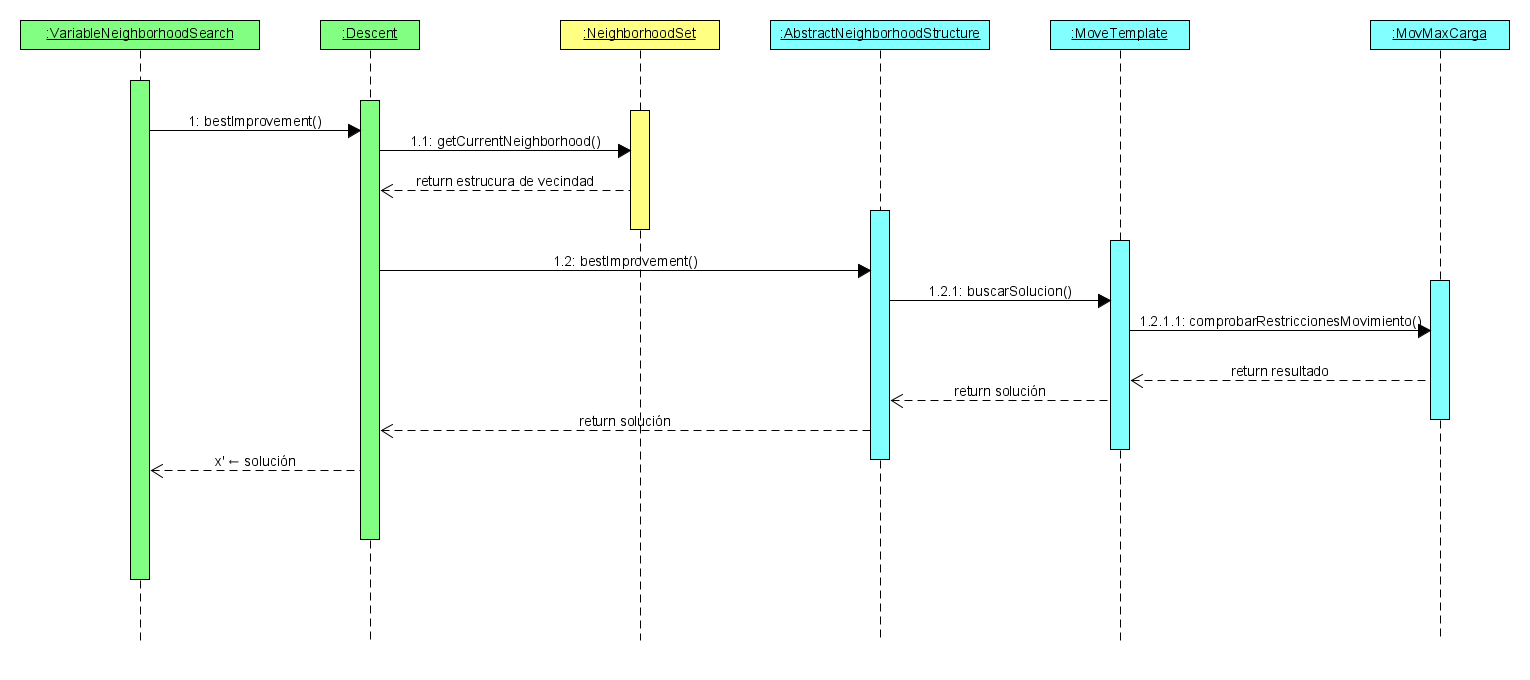
\includegraphics[width=\linewidth]{diagrama-interraccion}
	\caption{Diagrama de interacción de ejemplo.}
	\label{fig:B:diagrama-interraccion}
\end{figure}

\begin{landscape}
	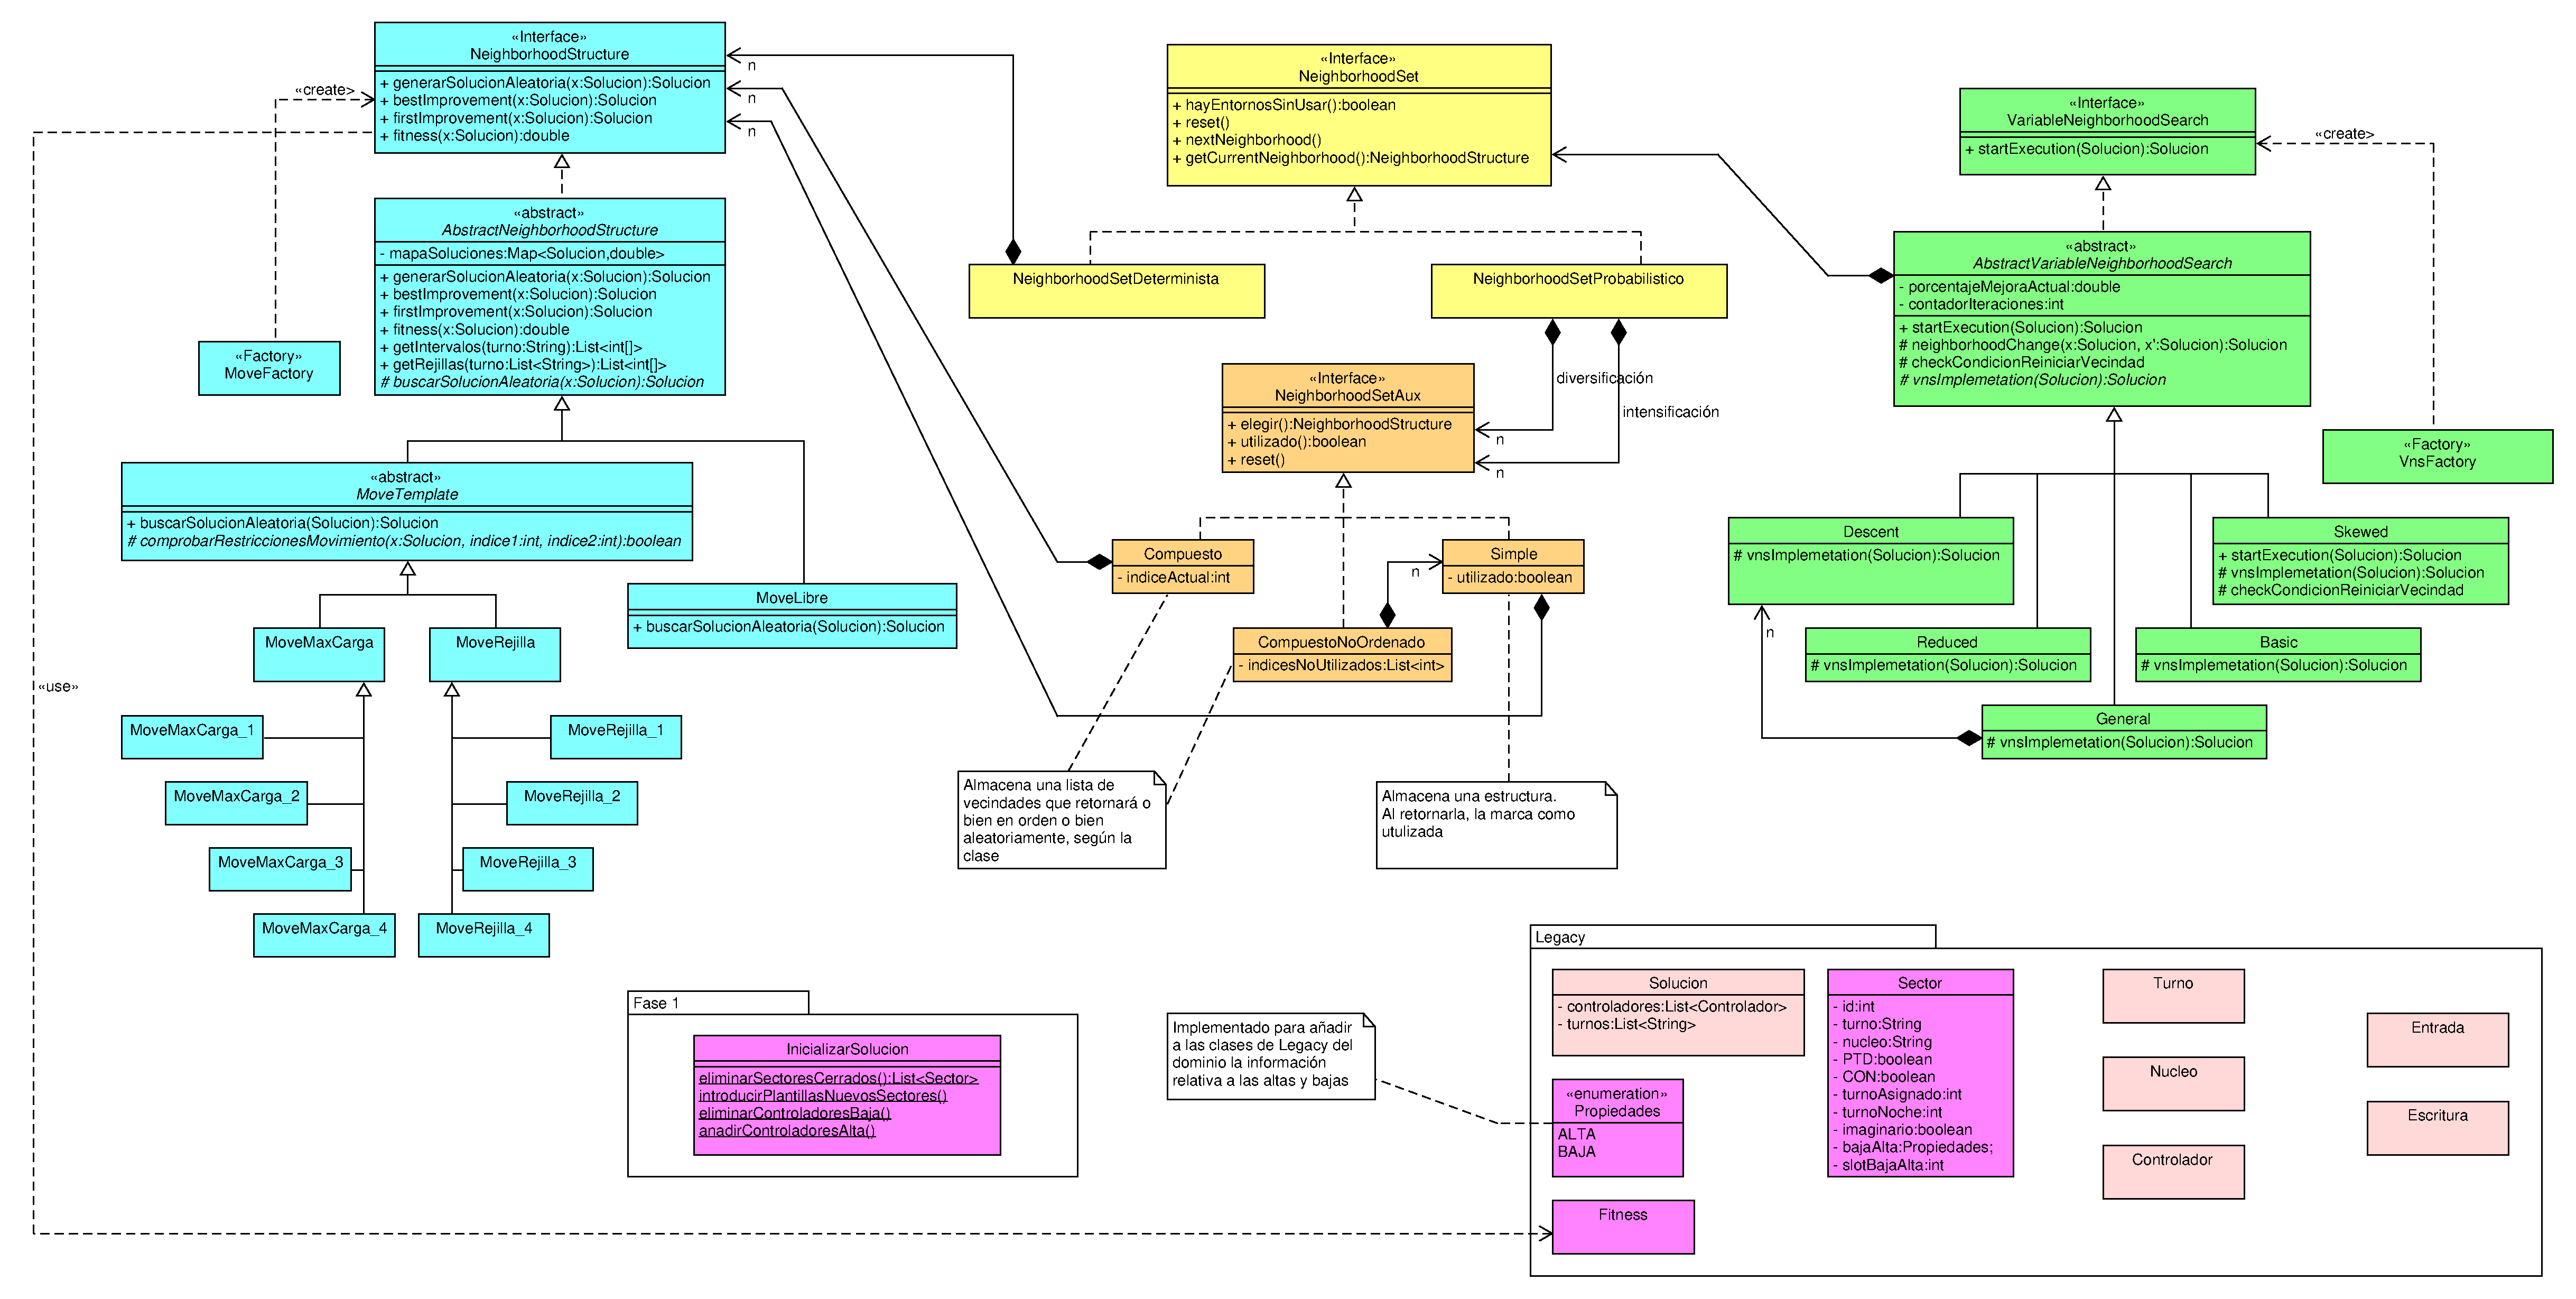
\includepdf[landscape=True]{diagrama-clases-completo}
\end{landscape}
